\chapter{Calculation of Condensed Field}

\section{Finding the Condensate of the Freeze-Out Surface}

The freeze-out surface is invariant under rotations (= independent of polar angle $\varphi$) around the collision axis and longitudinal boosts (= independent of rapidity $\eta_s$) and hence parametrized by a one-dimensional curve in the $r\text{-}\tau$-plane. The curve itself may be parametrized by some real parameter $\alpha$, following some mapping $s\mapsto (r(\alpha),\tau(\alpha))$. From the hydro simulation we wish to identify the gradient $\partial_\mu\vartheta\sim u_\mu$ of the complex phase of the condensate field with the fluid $4$-velocity $u_\mu$, hence in order to find the phase of the field, an integration of $\partial_\mu\vartheta$ over the hypersurface is needed and an integration constant $\vartheta_0$ can be chosen freely. Choose $\alpha=\arctan(y/x)$ to be the polar angle of the point $(r(\alpha),\tau(\alpha))$ in the $r\text{-}\tau$-plane. Since $r,\tau>0$ $\alpha$ is restricted to the range $[0,\pi]$ and $\vartheta(\alpha)$ on the hypersurface can be calculated via
\begin{equation}
    \vartheta(\alpha)=\vartheta_0+\int_0^\alpha\dt s\frac{\dt\vartheta}{\dt s}=\vartheta_0+\int_0^\alpha\dt s\frac{\partial x^\mu(s)}{\partial s}\partial_\mu\vartheta
\end{equation}
$\partial x^\mu(s)/\partial s$ represents the tangent vector of the freeze-out surface.

The energy density $\epsilon$ and $4$-velocity $u^\mu$ of the fluid is related to the condensate phase and density via
\begin{subequations}
    \begin{gather}
        -(\partial_\mu\vartheta)(\partial^\mu\vartheta)=\chi^2=\frac{-\mu^2+\sqrt{6\epsilon\lambda+2\mu^4}}{3}\\
        \partial^\mu\vartheta=\chi u^\mu\,,\qquad\rho^2=\sqrt{\frac{\chi^2+\mu^2}{\lambda}}
    \end{gather}
\end{subequations}
One may use the relations \eqref{eq:LinearSigmaModel_CouplingsMassesRelation} to rewrite the above equation in terms of the particle masses and the pion decay constant $f_\pi\equiv v$.
\begin{equation}
    \chi^2=\frac{-m_\sigma^2/2+\sqrt{3\epsilon m_\sigma^2/f_\pi+m_\sigma^4/2}}{3}=\frac{-m_\sigma^2+m_\sigma\sqrt{12\epsilon/f_\pi+2m_\sigma^2}}{6}\,,\qquad\rho=\sqrt{f_\pi\frac{2\chi^2+m_\sigma^2}{m_\sigma^2}}
\end{equation}

In Milne coordinates $(x^\mu)=(\tau,r,\varphi,\eta_s)$ the $4$-velocity has components $(u^\mu)=(\gamma,\gamma v,0,0)$, where $v=v(\alpha)$ is a function on the freeze-out surface.

Questions to Andreas regarding numerics:
\begin{itemize}
    \item Why is $\dt\alpha=\alpha_{j+1}-\alpha_{j}\neq\const$?
\end{itemize}

\section{Finding the Spectrum at the Detector Surface}

In general the particle number $N$ and particle number density $n(\mathbf{x})$ in position space and $n(\mathbf{p})$ in momentum space associated to the condensate $\phi(\mathbf{x})$ of a complex scalar field are given by the relations
\begin{subequations}
    \begin{gather}
        n(\mathbf{x})=\phi(\mathbf{x})\phi^*(\mathbf{x})\,,\qquad n(\mathbf{p})=\phi(\mathbf{p})\phi^*(\mathbf{p})\\
        N=\int\dt^3xn(\mathbf{x})=\int\frac{\dt^3p}{(2\pi)^3}n(\mathbf{p})
    \end{gather}
\end{subequations}
with the convention $\phi(\mathbf{x})=\int\dt^3p/(2\pi)^3\phi(\mathbf{p})e^{-\imagu\mathbf{p}\mathbf{x}}$ for the Fourier transform.



% The field configuration found by this translation prescription is then propagated forwards in time by means of the retarded Greens function
% \begin{equation}
%     \overline{\phi}(x)=\langle\phi_a(x)\rangle=\int\dt^dyG_{\text{ret}}(x,y)j(y)
% \end{equation}
% $j(y)$ is defined to be the field configruation on the freezout surface. The retarded Greens function is given by $G_{\text{ret}}(x,y)=\Theta(x^0-y^0)\big(D(x-y)-D(y-x)\big)$ where
% \begin{equation}
%     D(\Delta x)=\int\frac{\dt^3p}{(2\pi)^3}\frac{1}{2\omega_\mathbf{p}}e^{-\imagu(\omega_\mathbf{p}\Delta t-\mathbf{p}\Delta\mathbf{x})}
% \end{equation}
% and $\omega_\mathbf{p}=\sqrt{m^2+\mathbf{p}^2}$.

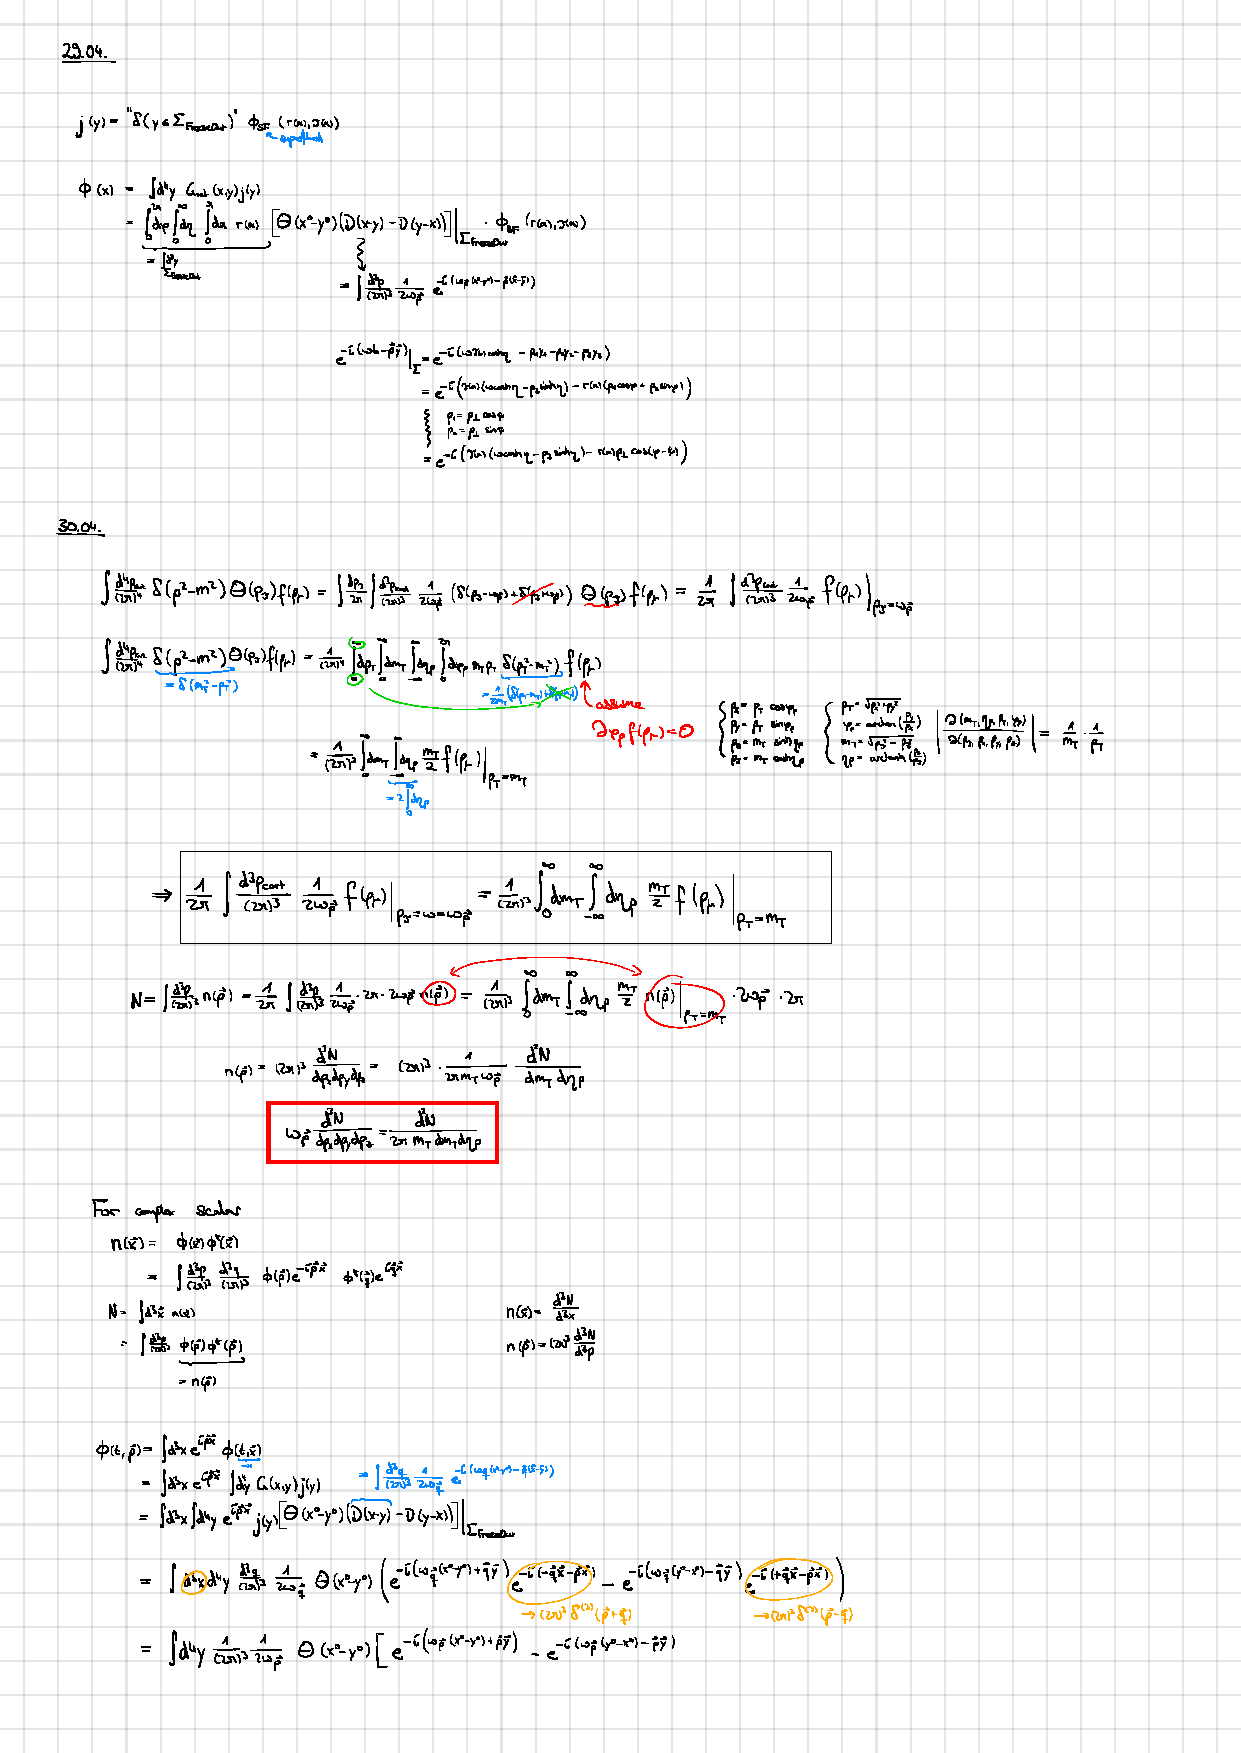
\includepdf{resources/notes_0430.pdf}
